\section{Мета роботи}
Отримати та закріпити знання про внутрішнє подання інтегрованих структур даних у мовах програмування.

\section{Хід роботи}
    Написати програму, яка виводить на екран внутрішнє подання
структури з варіантною частиною та з бітовими полями, а також масиву
структур. Перелік властивостей та відповідні типи полів для об’єктів з
табл. 4.1 обрати за своїм розсудом.

    Дослідити, як виконується вирівнювання даних та полів структури.
Порівняти час доступу до даних з вирівнюванням та за умови
відсутності вирівнювання. За результатами роботи підготувати звіт з
лабораторної роботи, де навести отримані результати та дати щодо них
пояснення, зробити висновки.

\begin{figure}[h!]
    \centering
    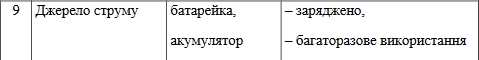
\includegraphics[width=14cm]{reports/algos/lab4/assets/1.png}
\end{figure}

\clearpage
\subsection{Ініціалізація структури}
Розглянемо створену мною структуру даних для лабораторної, у ній використовуються як бітові поля, так і варіативна частина:

\begin{figure}[h!]
    \centering
    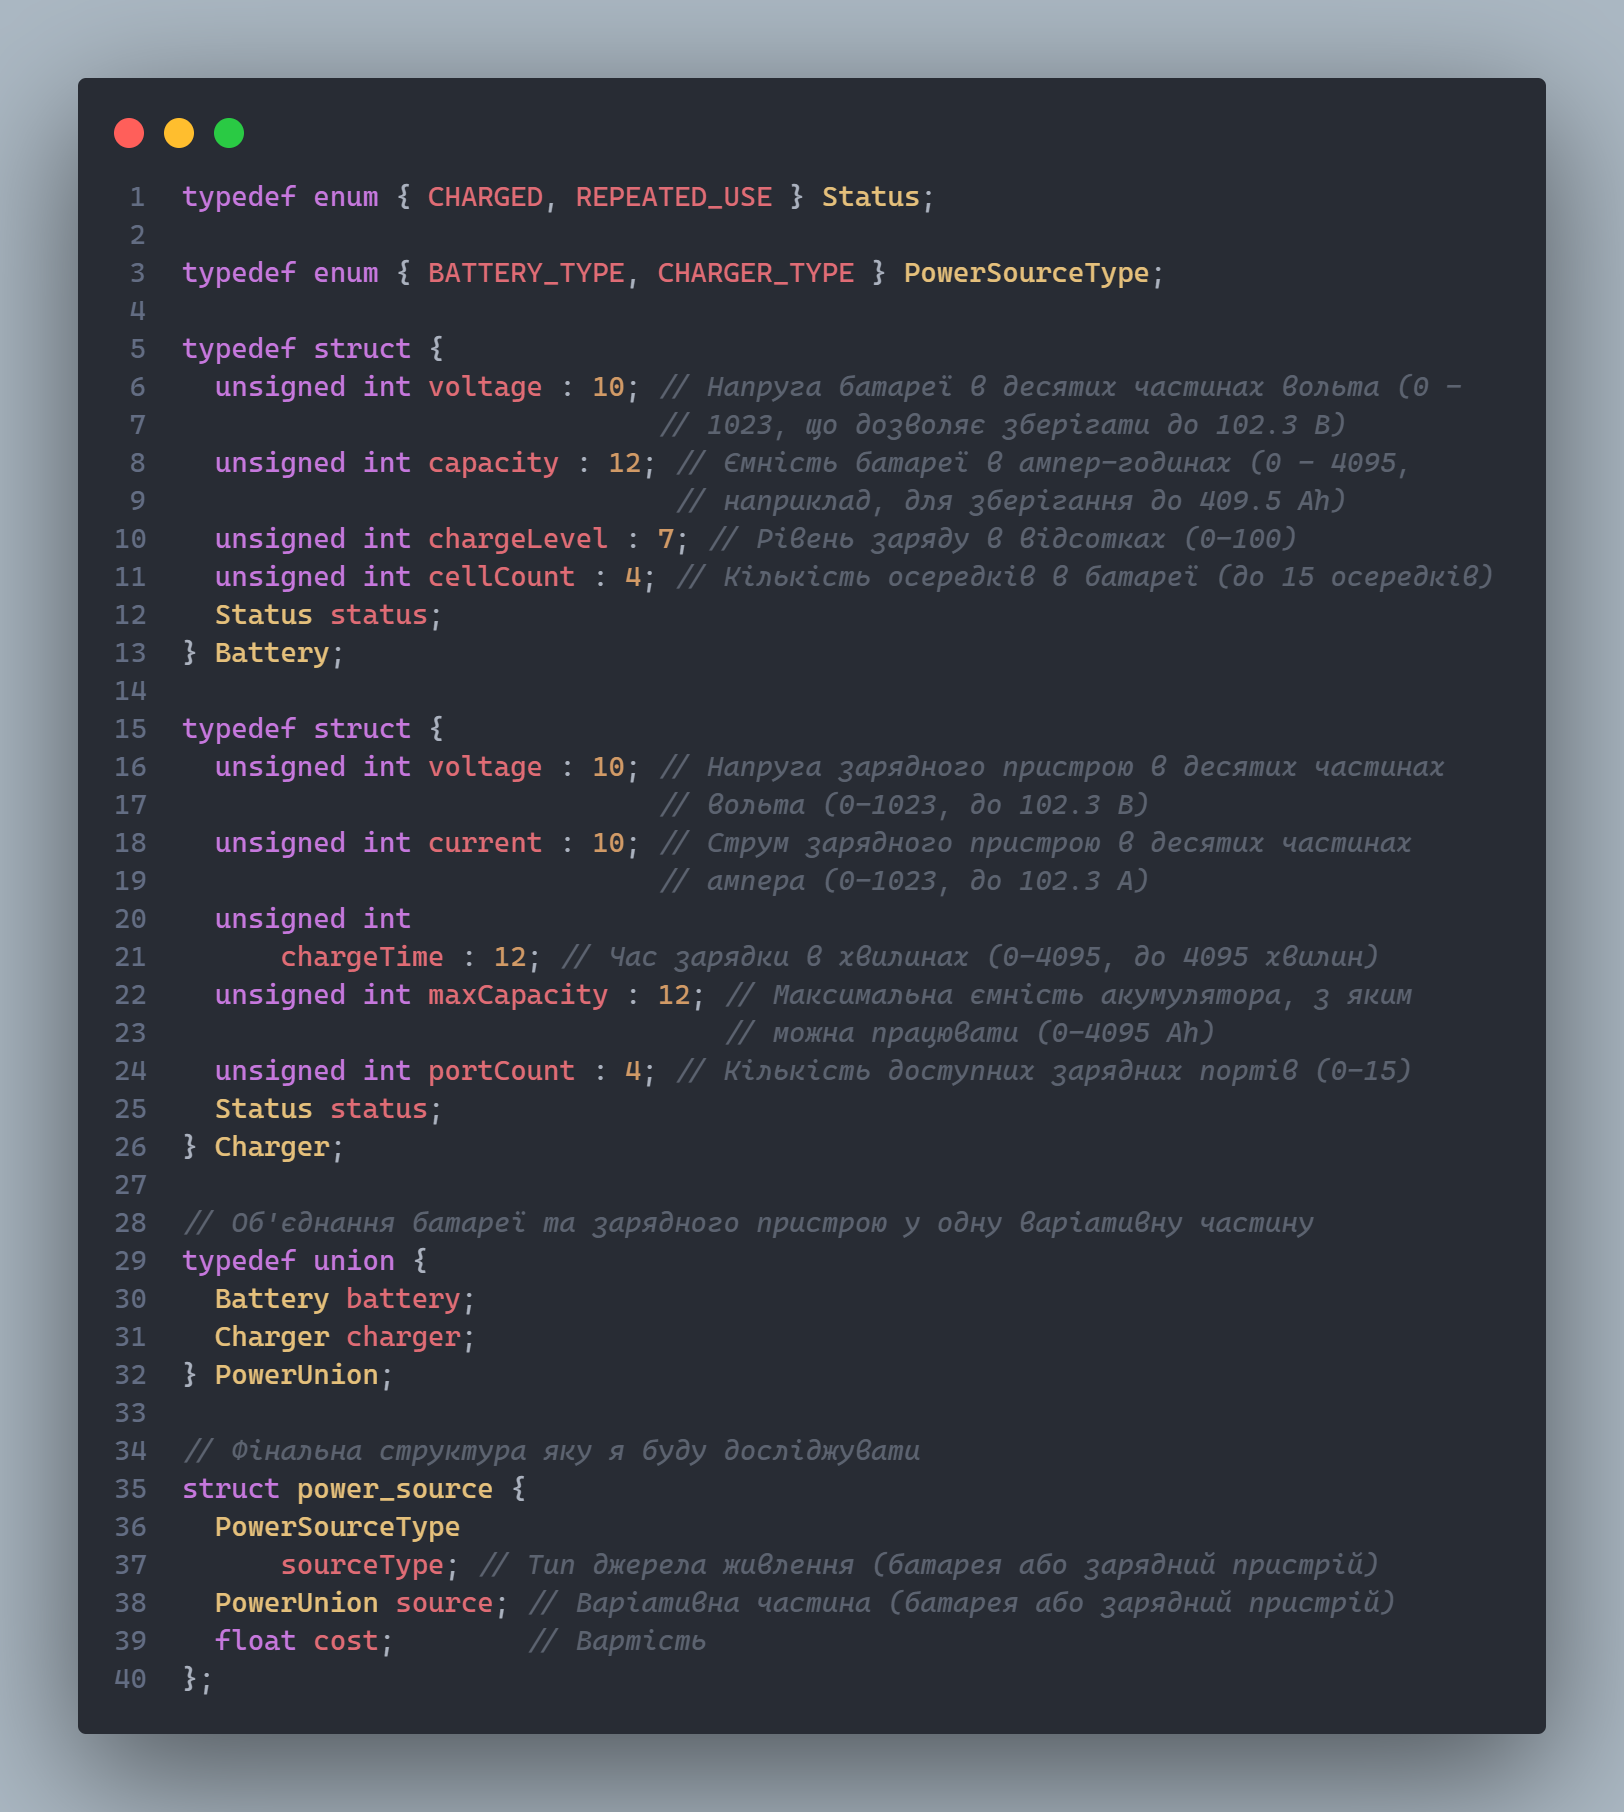
\includegraphics[width=18cm]{reports/algos/lab4/assets/2.png}
\end{figure}

\clearpage
\subsection{Машинний вигляд полів структури}

Спочатку створю змінну типу моєї структури та заповню її, після чого виведу значення кожного поля та його машинне представлення:

\begin{lstlisting}[style=customc]
void task1() {
  struct power_source batterySource = {
      BATTERY_TYPE, {.battery = {500, 3000, 80, 8, CHARGED}}, 150.0};

  highlightText("Field values of struct: ", "blue");
  print_struct_fields(&batterySource);
  printf("\n");

  highlightText("Machine representation of struct field values: ", "blue");
  print_binary_struct_fields(&batterySource);
  printf("\n");
};
\end{lstlisting}

\begin{figure}[h!]
    \centering
    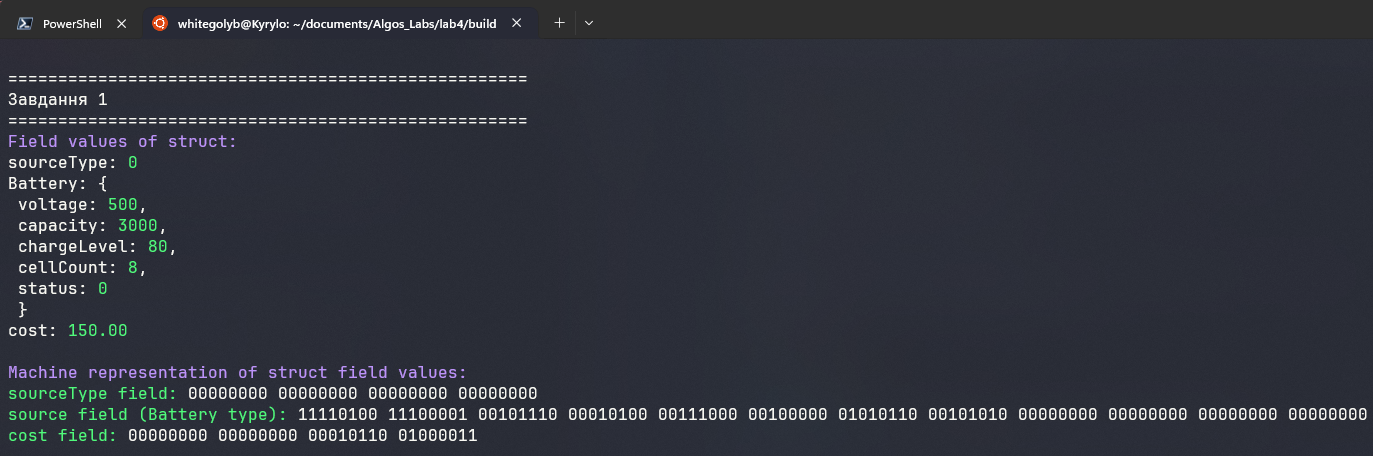
\includegraphics[width=18cm]{reports/algos/lab4/assets/3.png}
    \caption{Машинне представлення кожного поля структури}
\end{figure}

Після чого виведу представлення всієї структури разом у машинному вигляді за допомогою функції \textbf{print\_binary\_struct}:

\begin{lstlisting}[style=customc]
void print_binary_struct(void *ptr, size_t size) {
  unsigned char *byte = (unsigned char *)ptr;
  for (size_t i = 0; i < size; ++i) {
    printBinary(byte[i]);
  }
  printf("\n");
}

void task1() {
    struct power_source batterySource = {
        BATTERY_TYPE, {.battery = {500, 3000, 80, 8, CHARGED}}, 150.0};

    highlightText("Field values of struct: ", "blue");
    print_struct_fields(&batterySource);
    printf("\n");

    highlightText("Machine representation of struct field values: ", "blue");
    print_binary_struct_fields(&batterySource);
    printf("\n");

    highlightText("Machine representation of struct: ", "blue");
    print_binary_struct(&batterySource, sizeof(batterySource));
    printf("\n");
};
\end{lstlisting}

\begin{figure}[h!]
    \centering
    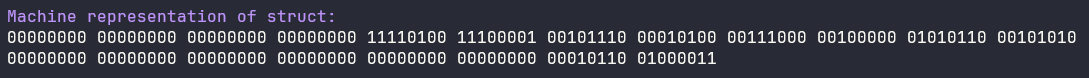
\includegraphics[width=18cm]{reports/algos/lab4/assets/4.png}
    \caption{Машинне представлення кожного поля структури}
\end{figure}

\subsection{Машинне представлення цілої структури}
Тепер створюю массив з 5 структур та виведу машинне представлення кожної структури в массиві структур у консоль:

\begin{lstlisting}[style=customc]
void print_internal_int(int val) {
  for (size_t i = 0; i < sizeof(int); i++) {
    printBinary((unsigned char)(val >> (i * 8)));
  }
  printf("\n");
}

void print_internal_float(float val) {
  unsigned char *floatBytes = (unsigned char *)&val;
  for (int i = 0; i < sizeof(float); i++) {
    printBinary(floatBytes[i]);
  }
  printf("\n");
}

void print_binary_struct(void *ptr, size_t size) {
  unsigned char *byte = (unsigned char *)ptr;
  for (size_t i = 0; i < size; ++i) {
    printBinary(byte[i]);
  }
  printf("\n");
}

void print_binary_array_of_struct(const struct power_source *arr, int size) {
  for (int i = 0; i < size; ++i) {
    printf("\033[32m%d)\033[0m ", i + 1);
    print_binary_struct(&arr[i], sizeof(arr[i]));
  }
  printf("\n");
}

void print_binary_struct_fields(const struct power_source *ps) {
  printf("\033[32msourceType field: \033[0m");
  print_internal_int(ps->sourceType);

  if (ps->sourceType == BATTERY_TYPE) {
    printf("\033[32msource field (Battery type): \033[0m");
    print_binary_struct(&ps->source.battery, sizeof(ps->source.battery));
  } else if (ps->sourceType == CHARGER_TYPE) {
    printf("\033[32msource field (Charger type): \033[0m");
    print_binary_struct(&ps->source.charger, sizeof(ps->source.charger));
  }

  printf("\033[32mcost field: \033[0m");
  print_internal_float(ps->cost);
}

void print_struct_fields(const struct power_source *ps) {
  printf("sourceType: \033[32m%d\033[0m\n", ps->sourceType);

  if (ps->sourceType == BATTERY_TYPE) {
    printf("Battery: { \n voltage: \033[32m%d\033[0m,\n capacity: "
           "\033[32m%d\033[0m,\n "
           "chargeLevel: \033[32m%d\033[0m,\n cellCount: "
           "\033[32m%d\033[0m,\n status: \033[32m%d\033[0m\n }\n",
           ps->source.battery.voltage, ps->source.battery.capacity,
           ps->source.battery.chargeLevel, ps->source.battery.cellCount,
           ps->source.battery.status);
  } else if (ps->sourceType == CHARGER_TYPE) {
    printf("Charger: { \n voltage: \033[32m%d\033[0m,\n current: "
           "\033[32m%d\033[0m,\n chargeTime: \033[32m%d\033[0m,\n "
           "maxCapacity: \033[32m%d\033[0m,\n portCount: "
           "\033[32m%d\033[0m,\n status: \033[32m%d\033[0m\n }\n",
           ps->source.charger.voltage, ps->source.charger.current,
           ps->source.charger.chargeTime, ps->source.charger.maxCapacity,
           ps->source.charger.portCount, ps->source.charger.status);
  }

  printf("cost: \033[32m%.2f\033[0m\n", ps->cost);
}

void task1() {
  struct power_source batterySource = {
      BATTERY_TYPE, {.battery = {500, 3000, 80, 8, CHARGED}}, 150.0};

  struct power_source items[5] = {
      {BATTERY_TYPE, {.battery = {600, 4000, 90, 10, CHARGED}}, 175.0},
      {CHARGER_TYPE, {.charger = {250, 600, 100, 2000, 3, REPEATED_USE}}, 60.0},
      {BATTERY_TYPE, {.battery = {450, 2500, 60, 6, CHARGED}}, 120.0},
      {CHARGER_TYPE, {.charger = {180, 400, 80, 1500, 2, REPEATED_USE}}, 45.0},
      {BATTERY_TYPE, {.battery = {550, 3500, 75, 7, CHARGED}}, 145.0}};

  highlightText("Field values of struct: ", "blue");
  print_struct_fields(&batterySource);
  printf("\n");

  highlightText("Machine representation of struct field values: ", "blue");
  print_binary_struct_fields(&batterySource);
  printf("\n");

  highlightText("Machine representation of struct: ", "blue");
  print_binary_struct(&batterySource, sizeof(batterySource));
  printf("\n");

  highlightText("Machine representation of array with structs: ", "blue");
  print_binary_array_of_struct(&items, 5);
};
\end{lstlisting}

\begin{figure}[h!]
    \centering
    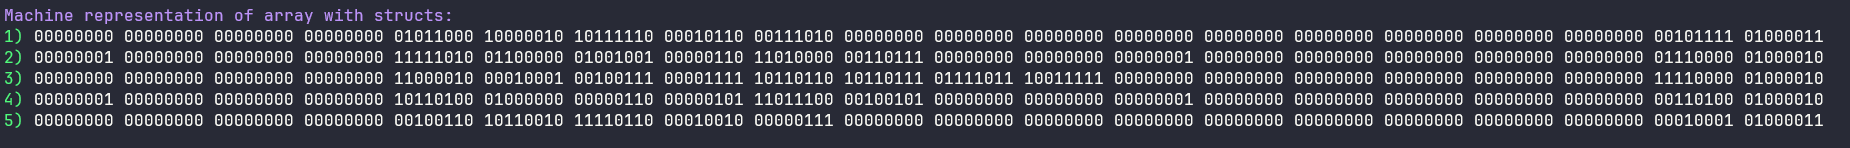
\includegraphics[width=18cm]{reports/algos/lab4/assets/5.png}
    \caption{Машинне представлення масиву структур}
\end{figure}

\begin{figure}[h!]
    \centering
    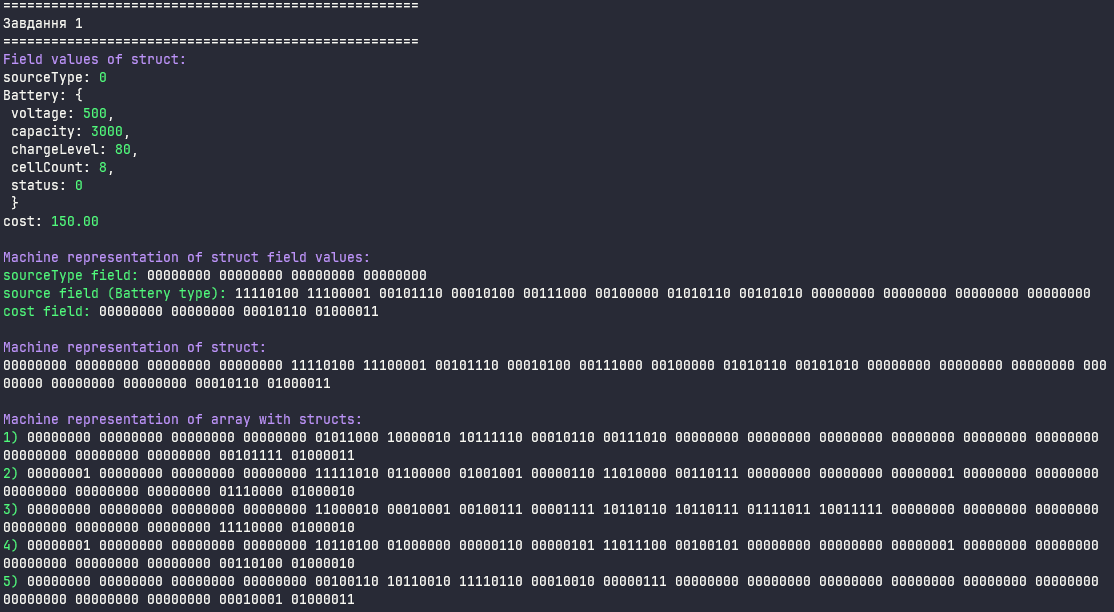
\includegraphics[width=18cm]{reports/algos/lab4/assets/6.png}
    \caption{Повний вивід результатів}
\end{figure}


\clearpage
\subsection{Порівняння швидкості доступу до структур з вирівнюванням та без вирівнювання}
Розмір структури з \textbf{вирівнюванням} становить 20 байт:
\begin{itemize}
    \item \textbf{sourceType} - int 4 байта
    \item \textbf{source \(Battery type\)} - структура з бітовими полями 12 байт
    \begin{itemize}
        \item \textbf{voltage} - 10 біт + 22 біт доповненя = 4 байта
        \item \textbf{capacity} - 12 біт + 4 біт доповнення = 2 байта
        \item \textbf{chargeLevel} - 7 біт + 1 біт доповнення = 1 байта
        \item \textbf{cellCount} - 4 біт + 4 біт доповнення = 1 байта
        \item \textbf{status} - int 32 біта = 4 байта
    \end{itemize}
    \item \textbf{cost} - float 4 байта
\end{itemize}

Для того щоб вимкнути вирівнювання на час досліду, до структур додаю додаткову строку у мові C: 

\begin{figure}[h!]
    \centering
    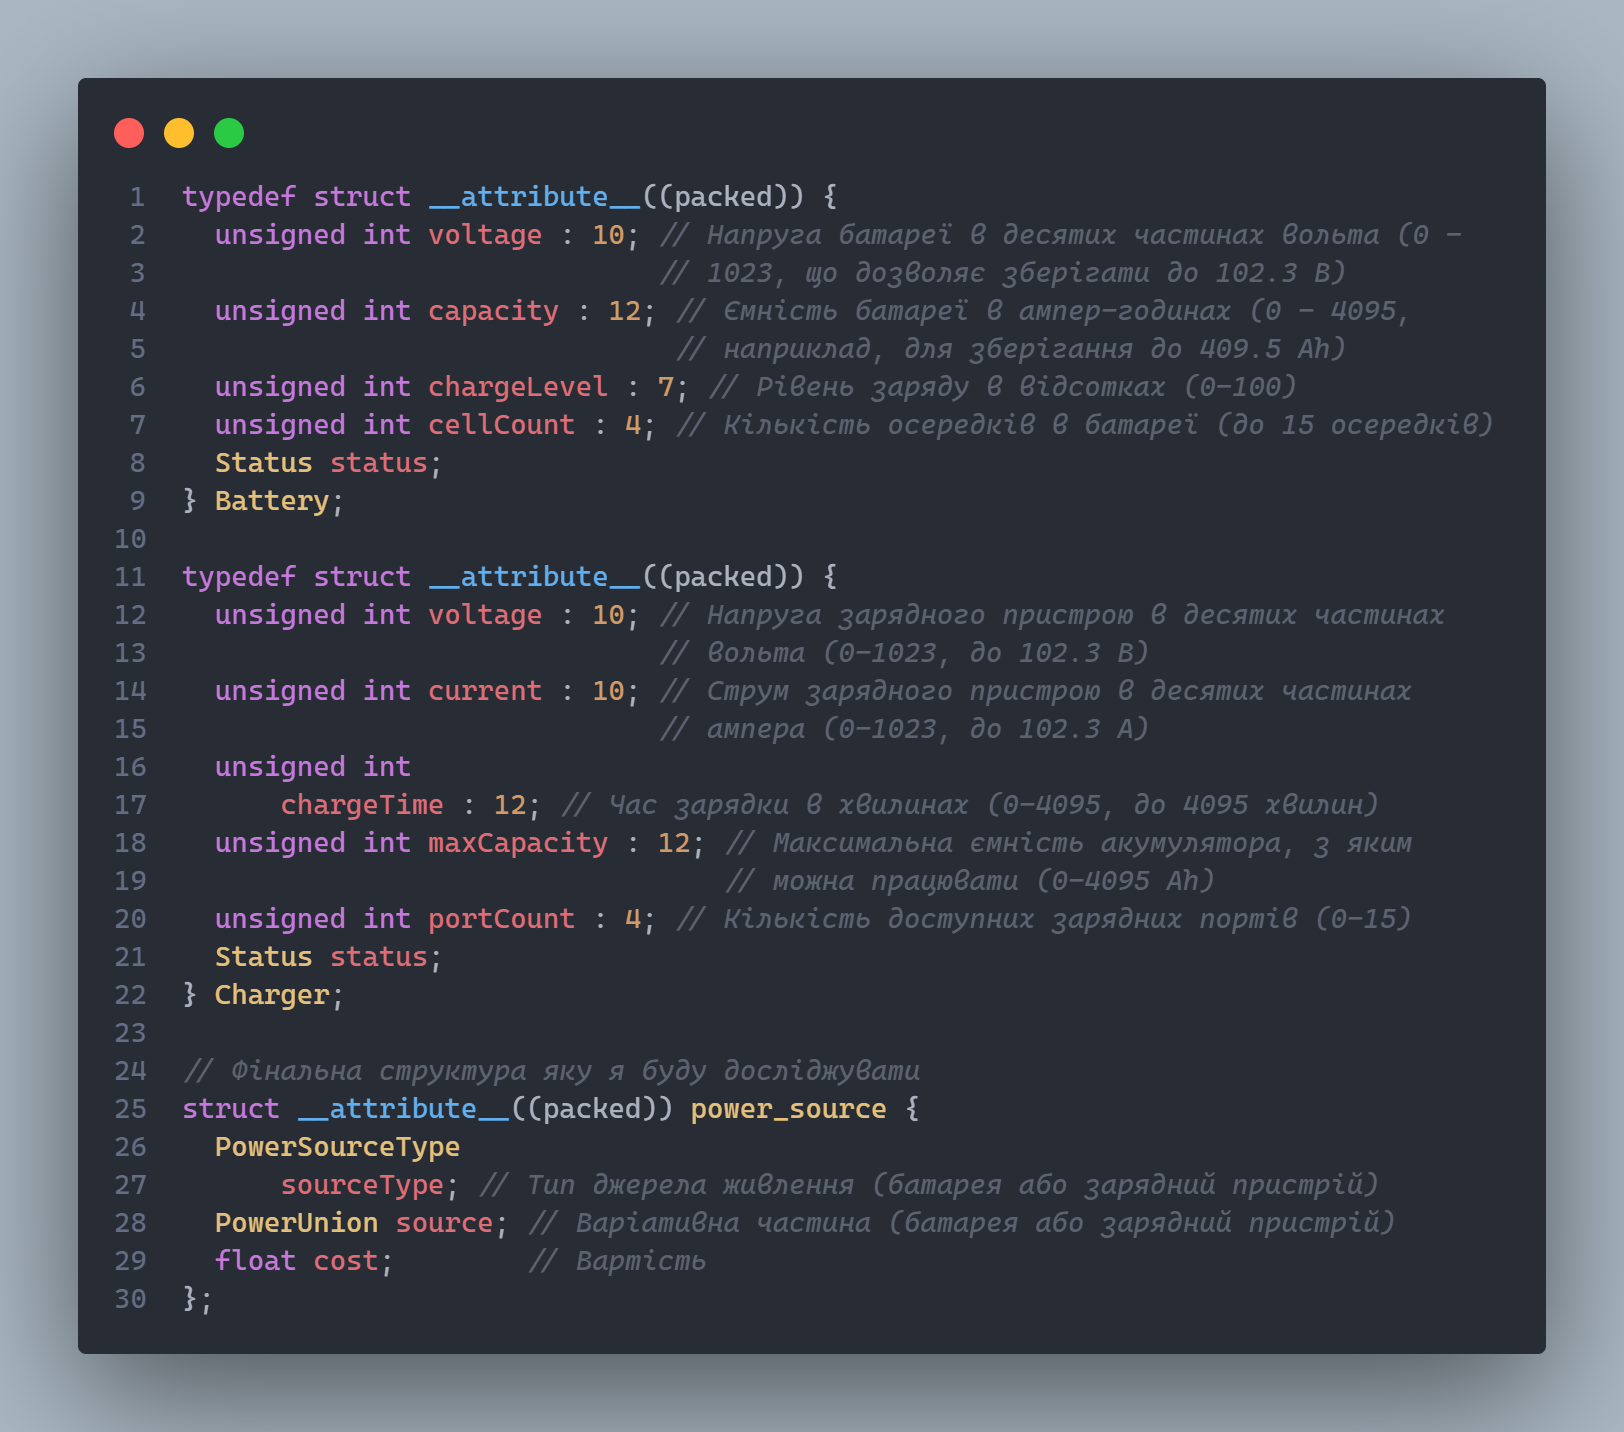
\includegraphics[width=14cm]{reports/algos/lab4/assets/7.png}
    \caption{Вимикання вирівнювання у структурах}
\end{figure}

\clearpage
Розмір структури \textbf{без вирівнювання} становить 18 байт:

\begin{itemize}
    \item \textbf{sourceType} - int 4 байта
    \item \textbf{source \(Battery type\)} - структура з бітовими полями 10 байт, тому що у PowerUnion саме більше поле це структура Charger - 10 байт без вирівнювання.
    \begin{itemize}
        \item \textbf{voltage} - 10 біт
        \item \textbf{capacity} - 12 біт
        \item \textbf{chargeLevel} - 7 біт
        \item \textbf{cellCount} - 4 біт
        \item \textbf{status} - int 32 біта
    \end{itemize}
    \item \textbf{cost} - float 4 байта
\end{itemize}

Тепер заміримо час доступу до полів структури \textbf{без вирівнювання та з ним}. Для отримання результатів я створив цикл що звертатиметься до її полів та запущу його мільярд разів, порахую середній час виконання:

\begin{lstlisting}[style=customc]
#include "general_utils.h"
#include <stdio.h>
#include <stdlib.h>
#include <time.h>

#define N 1000000000

void task1() {
  struct power_source batterySource = {
      BATTERY_TYPE, {.battery = {500, 3000, 80, 8, CHARGED}}, 150.0};

  highlightText(
      "Access time testing for structs with alignment and without it: ",
      "blue");

  clock_t start, end;
  double cpu_time_used;

  start = clock();

  for (int i = 0; i < N; i++) { 
    unsigned int v = batterySource.source.battery.voltage;
    unsigned int c = batterySource.source.battery.capacity;
    unsigned int cl = batterySource.source.battery.chargeLevel;
    unsigned int cc = batterySource.source.battery.cellCount;
    int s = batterySource.source.battery.status;

    (void)v; 
    (void)c;
    (void)cl;
    (void)cc;
    (void)s;
  }

  end = clock();

  cpu_time_used = ((double)(end - start)) / CLOCKS_PER_SEC;

  printf("Time for accessing struct fields (iterations \033[32m%d\033[0m): "
         "%.2f seconds\n",
         N, cpu_time_used);
};
\end{lstlisting}

Результати роботи програми:

\begin{figure}[h!]
    \centering
    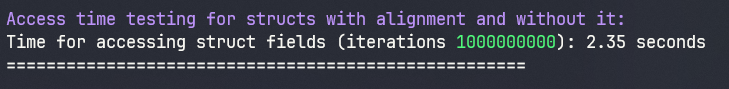
\includegraphics[width=14cm]{reports/algos/lab4/assets/8.png}
    \caption{Структура без вирівнювання}
\end{figure}

\begin{figure}[h!]
    \centering
    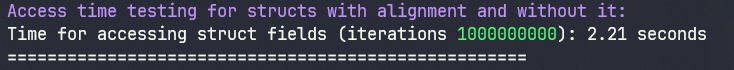
\includegraphics[width=14cm]{reports/algos/lab4/assets/9.png}
    \caption{Структура з вирівнюванням}
\end{figure}


\clearpage
\section{Висновки}
Під час виконання лабораторної роботи я навчився працювати зі структурами та представляти їх у машинному вигляді. Також розібрався з тим як працює вирівнювання на рівні компілятора та навіщо воно потрібно.
\\ 
\\
Після опрацювання отриманих результатів, можу зазначити що доступ до полів структури зі застосуванням вирівнювання здійснюється трішки швидше, ніж коли вирівнювання нема. Ці результати також можуть залежати від машини на якій відбувається код, але все ж таки бажано не вимикати вирівнювання задля забезпечення нормальної переносимості та сумісності програми з іншими пристроями, адже звертання до парних адрес комірок пам`яті відбувається швидше.

